\documentclass[conference]{IEEEtran}

\ifCLASSINFOpdf
   \usepackage[pdftex]{graphicx}

   \DeclareGraphicsExtensions{.pdf,.jpeg,.png,.gif,}
\else

\fi



\hyphenation{op-tical net-works semi-conduc-tor}


\begin{document}

\title{ Advance Ethernet}



\author{\IEEEauthorblockN{ARPAN CHAVDA}
\IEEEauthorblockA{09BCE006\\Department of Computer Science \& Engineering\\
Institute of Technology\\
Nirma University\\
Ahmedabad 382 481\\
Gujarat, India.\\ Email: 09BCE006@nirmauni.ac.in} \and
\IEEEauthorblockN{BHAVIN CHAUHAN}
\IEEEauthorblockA{09BCE005\\Department of Computer Science \& Engineering\\
Institute of Technology\\
Nirma University\\
Ahmedabad 382 481\\
Gujarat, India.\\
Email: 09BCE005@nirmauni.ac.in}}


\maketitle

\section{
{\LARGE Introduction}}
\IEEEpeerreviewmaketitle

\begin{itemize}
\item The Intel 8080 was the second 8-bit microprocessor designed and manufactured by Intel and was released in April 1974. It was an extended and enhanced variant of the earlier 8008 design, although without binary compatibility.\\

\item The initial specified clock freqency limit was 2 MHz and with common instructions having execution times of 4,5,7,10 or 11 cycles this meant a few hundred thousand instructions per second.\\


\item  The 8080 has sometimes been labeled "the first truly usable microprocessor", despite the fact that earlier microprocessors were used for calculators and other applications.\\

\end{itemize}
\begin{figure}[!h]
\begin{center}
%\rotatebox{100}
{\scalebox{0.11}{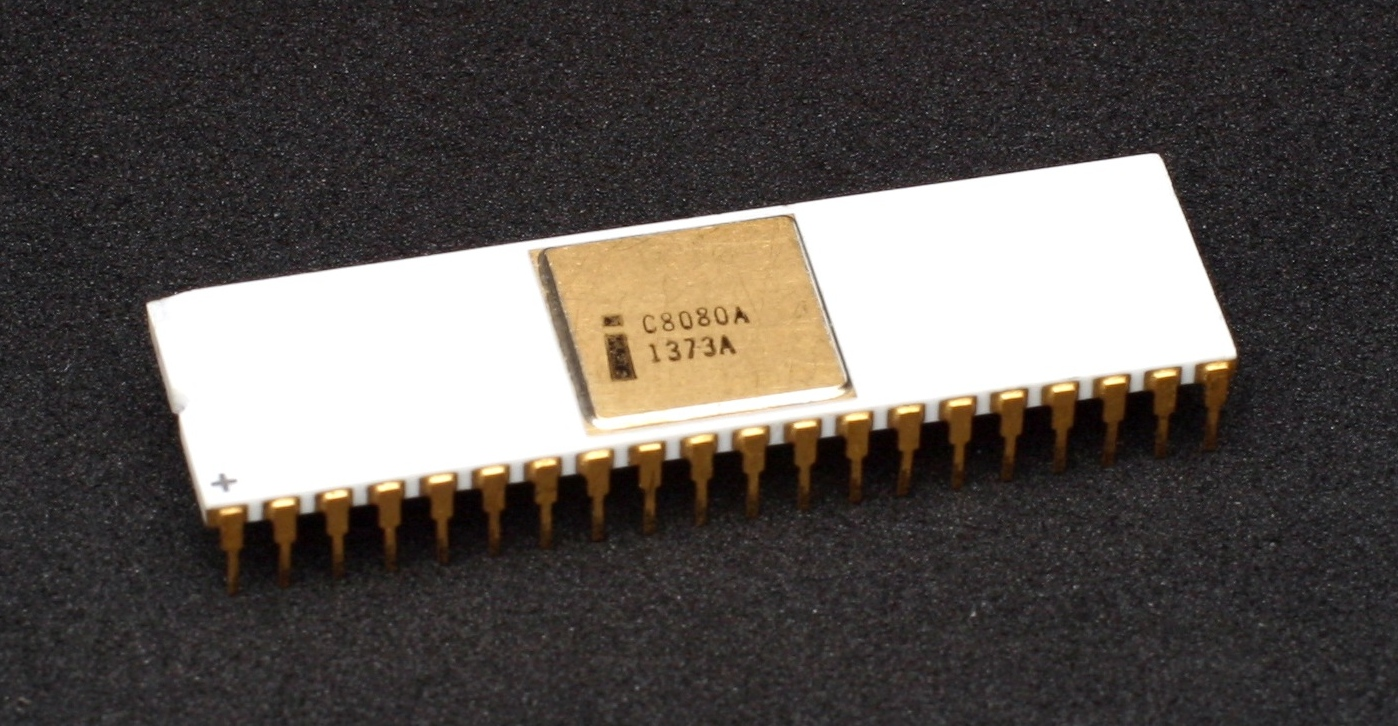
\includegraphics{8080.jpg}}}
\caption{Intel 8080 Chip}
\end{center}
\end{figure}

\section{
{\LARGE Architecture}}

{\large Memory}
\begin{itemize}
\item Program, data and stack memories occupy the same memory space. The total addressable memory size is 64 KB.

\item Program memory - program can be located anywhere in memory. Jump, branch and call instructions use 16-bit addresses, i.e. they can be used to jump/branch anywhere within 64 KB. All jump/branch instructions use absolute addressing.

\item Data memory - the processor always uses 16-bit addresses so that data can be placed anywhere.

\item Stack memory is limited only by the size of memory. Stack grows downward.\\
\end{itemize}
{\large Registers}
\begin{itemize}

\item Accumulator or A register is an 8-bit register used for arithmetic, logic, I/O and load/store operations.\\

\item Flag is an 8-bit register containing 5 1-bit flags:\\


\item {\small General registers:}

    - 8-bit B and 8-bit C registers can be used as one 16-bit BC register pair. When used as a pair the C register contains low-order byte. Some instructions may use BC register as a data pointer.\\
    - 8-bit D and 8-bit E registers can be used as one 16-bit DE register pair. When used as a pair the E register contains low-order byte. Some instructions may use DE register as a data pointer.\\
    - 8-bit H and 8-bit L registers can be used as one 16-bit HL register pair. When used as a pair the L register contains low-order byte. HL register usually contains a data pointer used to reference memory addresses.\\

\item Stack pointer is a 16 bit register. This register is always incremented/decremented by 2.\\

\item Program counter is a 16-bit register.\\
\end{itemize}
{\large Input/Output Ports}
\begin{itemize}
\item 256 Input ports and 256 Output Ports\\
\end{itemize}

{\large \newpage Addressing modes}
\begin{itemize}



\item Register-references the data in a register or in a register pair.\\
\item Register indirect-instruction specifies register pair containing address, where the data is located.\\
\item Direct.\\
\item Immediate - 8 or 16-bit data.\\\\
\end{itemize}

\begin{figure}[!h]
\begin{center}
%\rotatebox{100}
{\scalebox{0.7} {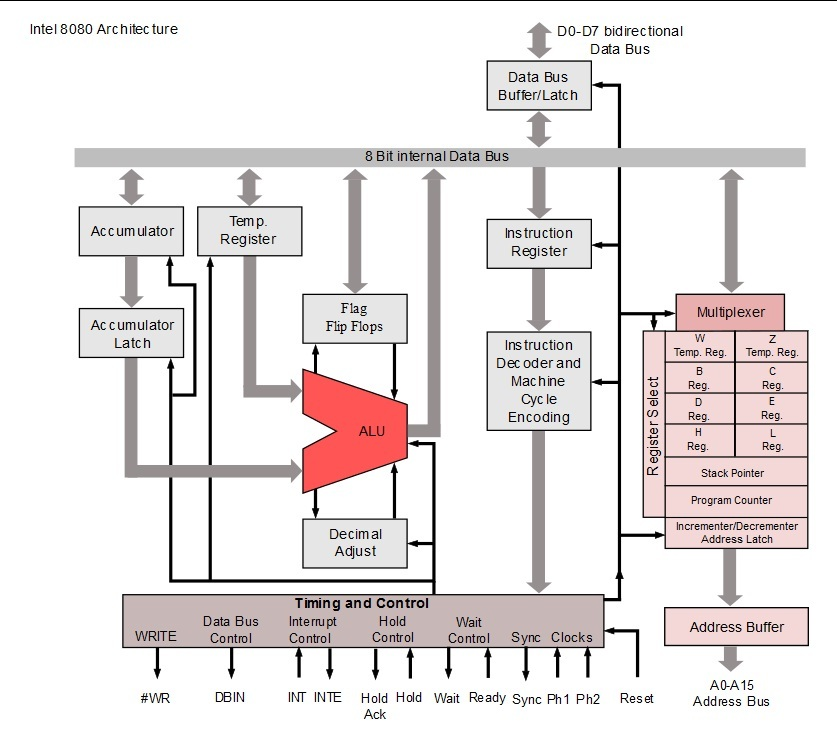
\includegraphics{8081.jpg}}}
\caption{Intel 8080 Architecture}
\end{center}
\end{figure}

{\newpage \large Instruction Set:}
 8080 instruction set consists of the following instructions:\\
\begin{itemize}

    \item Data moving instructions.
    \item Arithmetic - add, subtract, increment and decrement.
    \item Logic - AND, OR, XOR and rotate.
    \item Control transfer - conditional, unconditional, call subroutine, return from subroutine and restarts.
    \item Input/Output instructions.
    \item Other - setting/clearing flag bits, enabling/disabling interrupts, stack operations, etc.

    \end{itemize}
\newpage

\begin{figure}[!h]
\begin{center}
%\rotatebox{100}
{\scalebox{0.9} {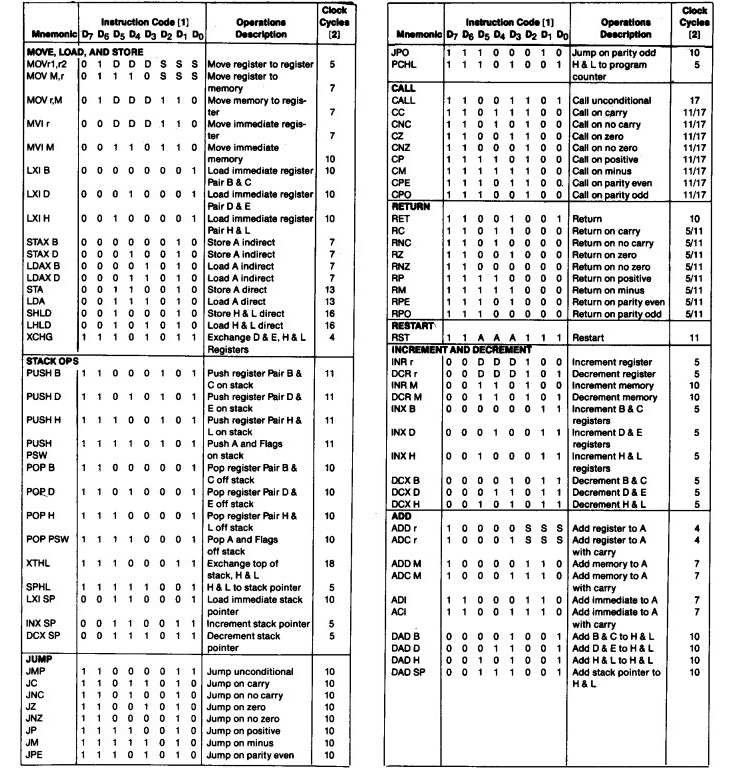
\includegraphics{in1.jpg}}}
\caption{Intructions-1}
\end{center}
\end{figure}\newpage\clearpage
\begin{figure}[!h]
\begin{center}
%\rotatebox{100}
{\scalebox{0.9} {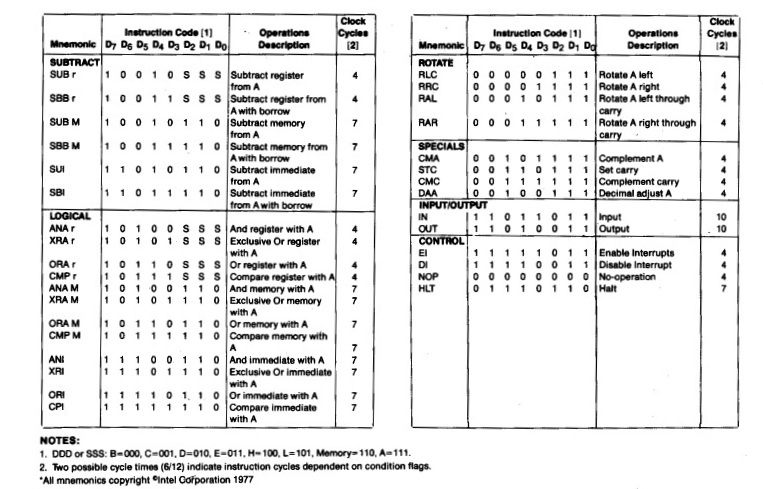
\includegraphics{in2.jpg}}}\newpage
\caption{Intructions-2}
\end{center}
\end{figure}\newpage
\subsection\newpage{THE PROCESSOR STATUS REGISTER (FLAGS)}
\begin{figure}[!h]
\begin{center}
%\rotatebox{200}
{\scalebox{0.8} {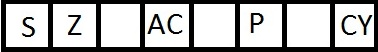
\includegraphics{flg.jpg}}}
\caption{Flag Register}
\end{center}
\end{figure}
\begin{enumerate}
    \item Sign - set if the most significant bit of the result is set.\\
    \item Zero - set if the result is zero.\\
    \item Auxiliary carry - set if there was a carry out from bit 3 to bit 4 of the result.\\
    \item Parity - set if the parity (the number of set bits in the result) is even.\\
    \item Carry - set if there was a carry during addition, or borrow during subtraction/comparison.\\
\end{enumerate}
\section{{\large PIN DIAGRAM}}
\begin{figure}[!h]
\begin{center}
%\rotatebox{200}
{\scalebox{0.5} {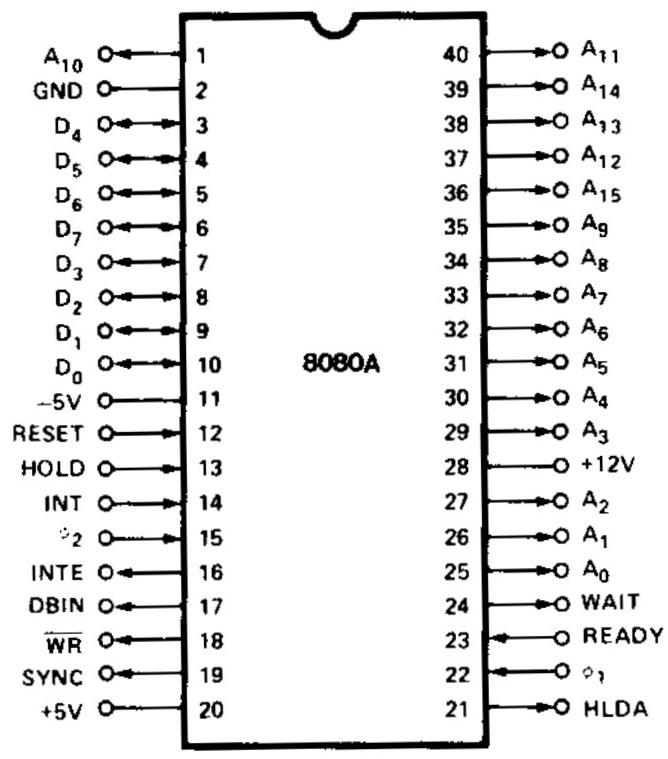
\includegraphics{pin.jpg}}}
\caption{Pin Diagram of 8080A}
\end{center}
\end{figure}
\begin{figure}[!h]
\begin{center}
%\rotatebox{200}
{\scalebox{0.5} {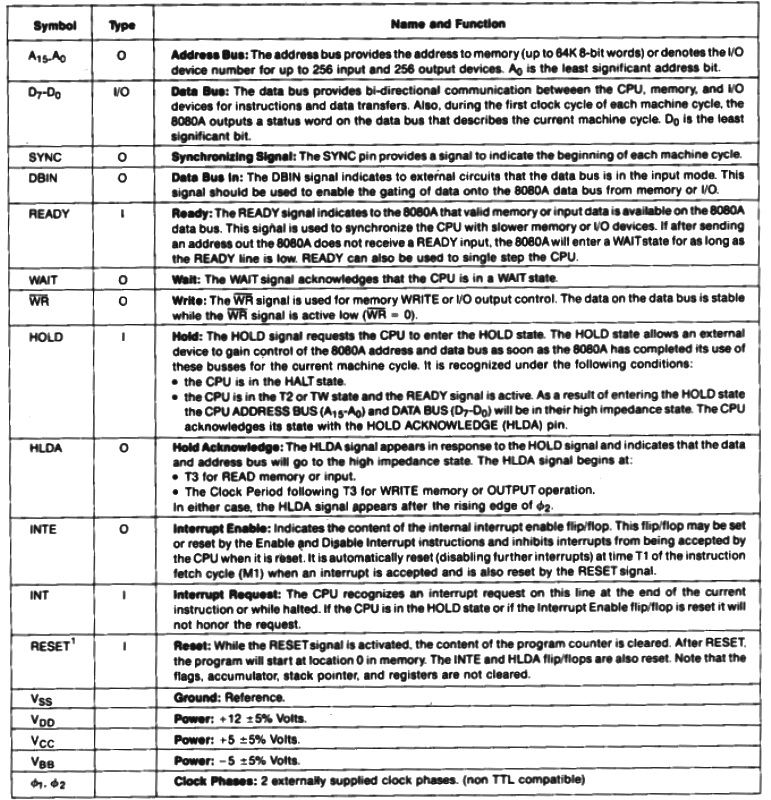
\includegraphics{pinfn.jpg}}}
\caption{Pin Functions of 8080A}
\end{center}
\end{figure}
\clearpage
\section{\large THE INDUSTRIAL IMPACT}
\begin{itemize}
\item The 8080 was used in many early microcomputers, such as the MITS Altair 8800 Computer, Processor Technology SOL-20 Terminal Computer and IMSAI 8080 Microcomputer, forming the basis for machines running the CP/M operating system.
\item The 8080 was actually designed for just about any application except a complete computer system. Hewlett Packard developed the HP 2640 series of smart terminals around the 8080. The HP 2647 was a terminal which ran BASIC on the 8080.
\item In addition, several early arcade video games were built around the 8080 microprocessor. Space Invaders was perhaps the most popular such title.\\
\end{itemize}
\newpage

\section{\large REFERENCE }
\begin{itemize}
\item Wikipedia,The free Encyclopedia
\item MICROCOMPUTERS AND MICROPROCESSORS(2nd EDITION) BY JOHN UFFENBECK
\item Intel 8080 Microprocessor Datasheet
\end{itemize}



\end{document}
